\section{PC104}
\label{pc104}


\begin{table}[ht!]

	\begin{tabular}{r l|l p{12cm} }
		
		\textcolor{gray}{Especificação} &&& 	{ADLD25PC-525 - Atom Dual Core D525,
		1.80GHz}\\
		\textcolor{gray}{Data} &&& 				{31/07/2014}\\
        \textcolor{gray}{Beneficiado} &&&		{ADL Embedded Solutions Inc.} \\
        \textcolor{gray}{CNPJ} &&& 				{Internacional} \\
        \textcolor{gray}{Número Nota} &&& 		{ORS37752} \\
		\textcolor{gray}{Quantidade} &&& 		{1} \\
		\textcolor{gray}{Valor} &&& 			{R\$3.778,95} \\
		\textcolor{gray}{Data Sheet} &&& 		{Anexo VI - \ref{datasheet_pc104}} \\

		\textcolor{gray}{Função no projeto} &&& {O PC104 será utilizado na eletrônica
		de superfície (base) ou como segunda opção para a eletrônica embarcada
		(proposta 3). É responsável por se comunicar com a eletrôncia embarcada por
		Ethernet.}
		\\
		\textcolor{gray}{Razão da Escolha} &&& {Fornecedor mais reconhecido no
		mercado para módulos PC104.}
	\end{tabular}
\end{table}

\newpage

\subsection{Foto do Material}
\begin{figure}[H]
 \centering
 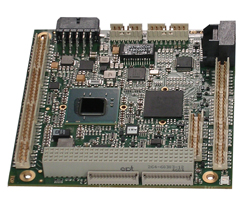
\includegraphics[width=1\columnwidth]{PC104/foto.jpg}
 \caption{PC104}
\end{figure} 

\subsection{Nota Fiscal}
\begin{figure}[H]
 \centering
 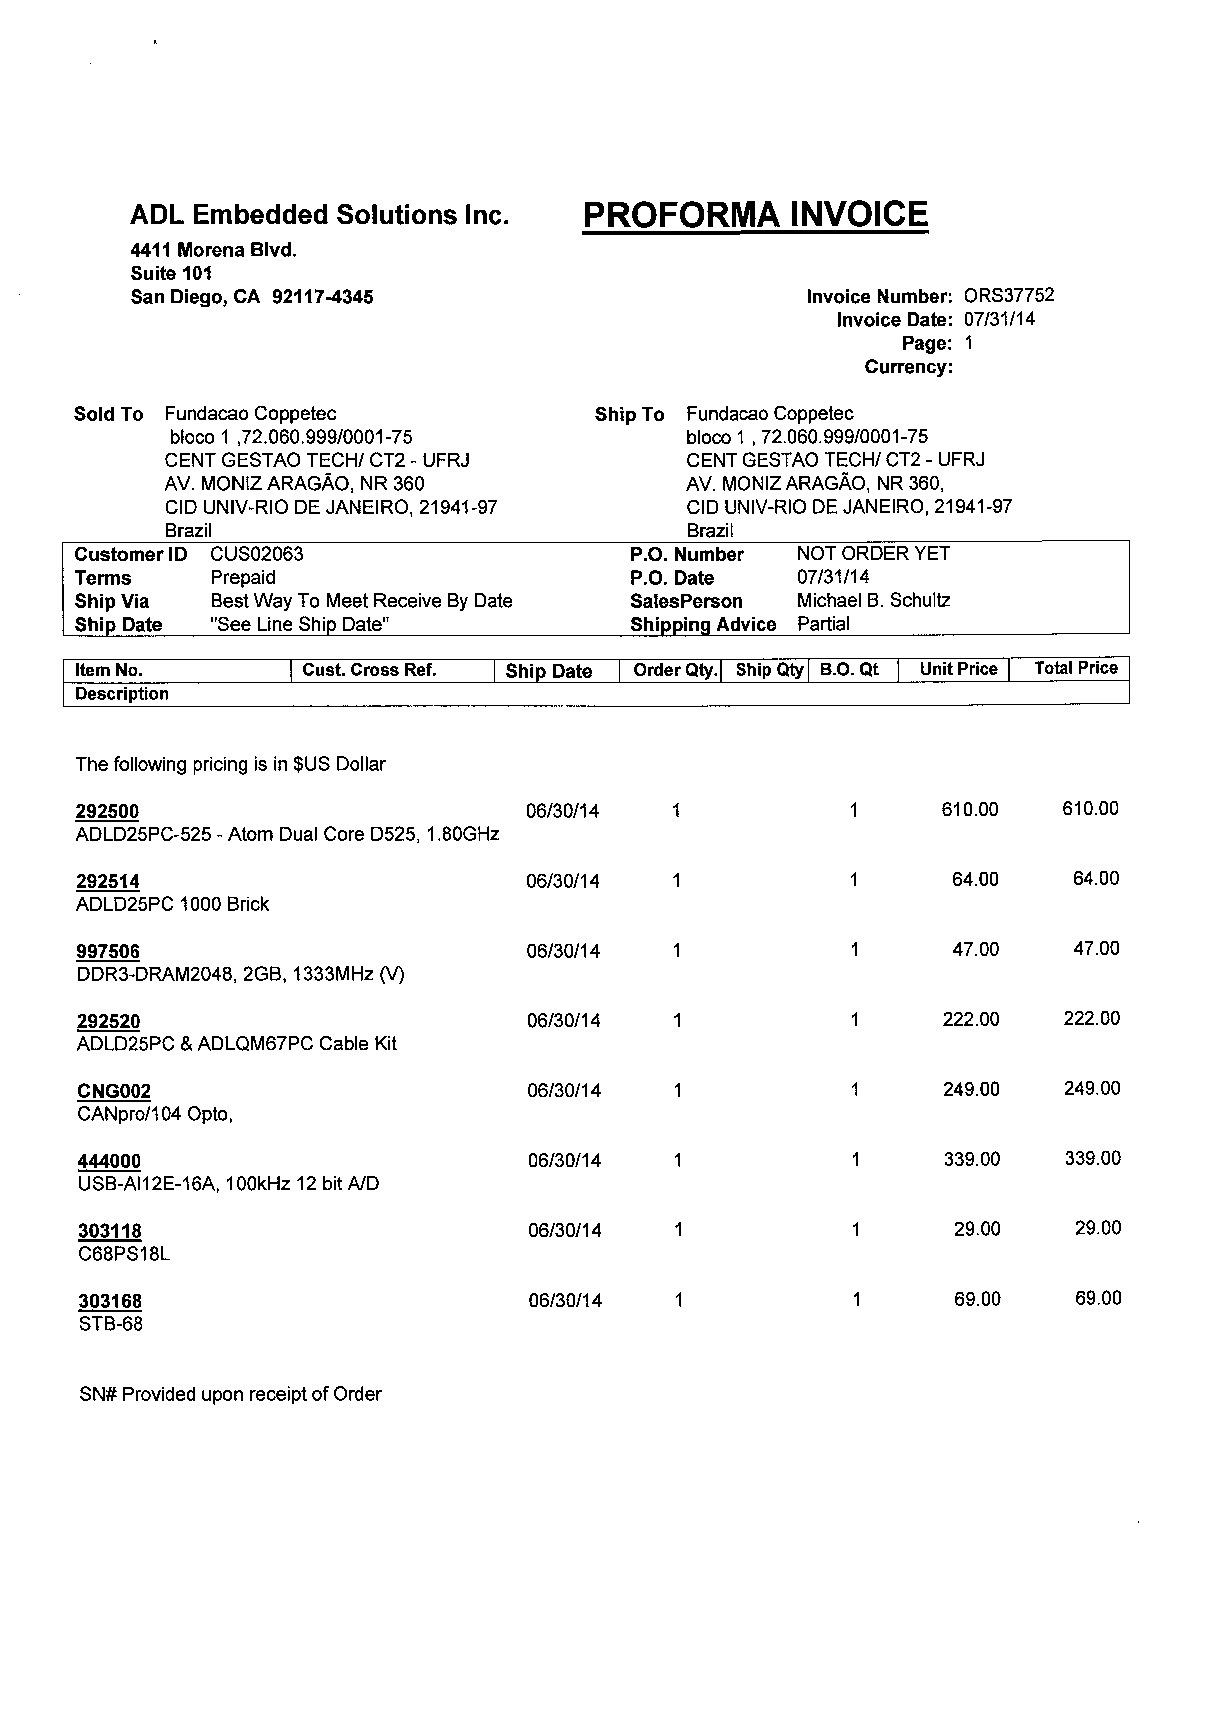
\includegraphics[width=0.9\columnwidth]{PC104/nota_adl.pdf}
 \caption{Nota fiscal do PC104}
\end{figure}


